\documentclass{beamer}

\setbeamertemplate{frametitle}[default][center]
\usepackage[size=a4]{beamerposter}
% remove nav symbols
\setbeamertemplate{navigation symbols}{}

\usepackage{scrextend}
\changefontsizes{18pt}
  % package to use double spacing
  \usepackage{setspace}

  
  % \usepackage{tikz}
  
  % % neural network
  % \usetikzlibrary{matrix,chains,positioning,decorations.pathreplacing,arrows}
  
  
  
  % package to add wrapfigure
  \usepackage{wrapfig}
  
  
  % package to add graphs
  \usepackage{pgfplots}
  
  % packages to add images
  \usepackage{graphicx}
  
  
  \begin{document}
  % \pgfplotsset{compat=1.15}

  \begin{frame}
    \frametitle{Objectives}

    % Research Question
    % Whilst the use of evolutionary algorithms and neural networks have been explored independently of one another to create draughts players, the intention is to explore the effectiveness of the combined methods in developing an artificially intelligent draughts playing agent. 


    \begin{block}{Minimum Objective}
      The minimum objective was to implement a feed-forward neural network, and a genetic algorithm that interacted with the neural network, allowing it to improve over time. This would need to be connected to a Draughts Interface that allowed the neural network to play Draughts. 
      % This was achieved by having each component implemented manually in Python and the NumPy library.

      \end{block}

        
    \begin{block}{Intermediate Objective}
        % The intermediate objective of this project was to create and incorporate the algorithms for the calculation of triangle surface normals, vertex normals and gradient (following our definition) in the initial programme, and enable visualisation of the “interesting” gradient changes and vertex normals on the mesh displayed by the programme.
        The intermediate objective involved the implementation of an interface to play against the trained result, and the implementation of a Monte-Carlo Tree-Search (MCTS) algorithm. Also, as the genetic algorithm included a tournament mechanism which would play games simultaneously, this needed to be implemented to run in parallel.
        % The implementation of the tournament mechanism was made possible via the use of a round robin approach and the use of the multiprocessing Python library. MCTS was successfully implemented, which improved the system's ability to choose moves.
        
      \end{block}

        
    \begin{block}{Advanced Objective}
        % The advanced objective of this project was to evaluate the speed of the algorithms and compare it to the time complexity that we obtained from theoretical analysis of the algorithms. The final sections of this paper will show the results acquired and the analysis and evaluation of the work we carried out. 
        The advanced objective consisted of producing a system showing indications that it was learning over time. Measurements were taken to determine whether the genetic algorithm improved the neural network, and which properties of the genetic algorithm made it possible.
    
      \end{block}

        
  \end{frame}


  \begin{frame}
    \frametitle{Objectives}

    % Research Question
    % Whilst the use of evolutionary algorithms and neural networks have been explored independently of one another to create draughts players, the intention is to explore the effectiveness of the combined methods in developing an artificially intelligent draughts playing agent. 


    \begin{block}{Minimum Objective}
      The minimum objective was to implement a feed-forward neural network, and a genetic algorithm that interacted with the neural network, allowing it to improve over time. This would need to be connected to a Draughts Interface that allowed the neural network to play Draughts. 
      % This was achieved by having each component implemented manually in Python and the NumPy library.

      \end{block}

        
    \begin{block}{Intermediate Objective}
        % The intermediate objective of this project was to create and incorporate the algorithms for the calculation of triangle surface normals, vertex normals and gradient (following our definition) in the initial programme, and enable visualisation of the “interesting” gradient changes and vertex normals on the mesh displayed by the programme.
        The intermediate objective involved the implementation of an interface to play against the trained result, and the implementation of a Monte-Carlo Tree-Search (MCTS) algorithm. Also, as the genetic algorithm included a tournament mechanism which would play games simultaneously, this needed to be implemented to run in parallel.
        % The implementation of the tournament mechanism was made possible via the use of a round robin approach and the use of the multiprocessing Python library. MCTS was successfully implemented, which improved the system's ability to choose moves.
        
      \end{block}

        
    \begin{block}{Advanced Objective}
        % The advanced objective of this project was to evaluate the speed of the algorithms and compare it to the time complexity that we obtained from theoretical analysis of the algorithms. The final sections of this paper will show the results acquired and the analysis and evaluation of the work we carried out. 
        The advanced objective consisted of producing a system showing indications that it was learning over time. Measurements were taken to determine whether the genetic algorithm improved the neural network, and which properties of the genetic algorithm made it possible.
    
      \end{block}

        
  \end{frame}

  \begin{frame}
    \frametitle{Cummulative Growth} 
    \begin{figure}[!ht]
      
      \centering
      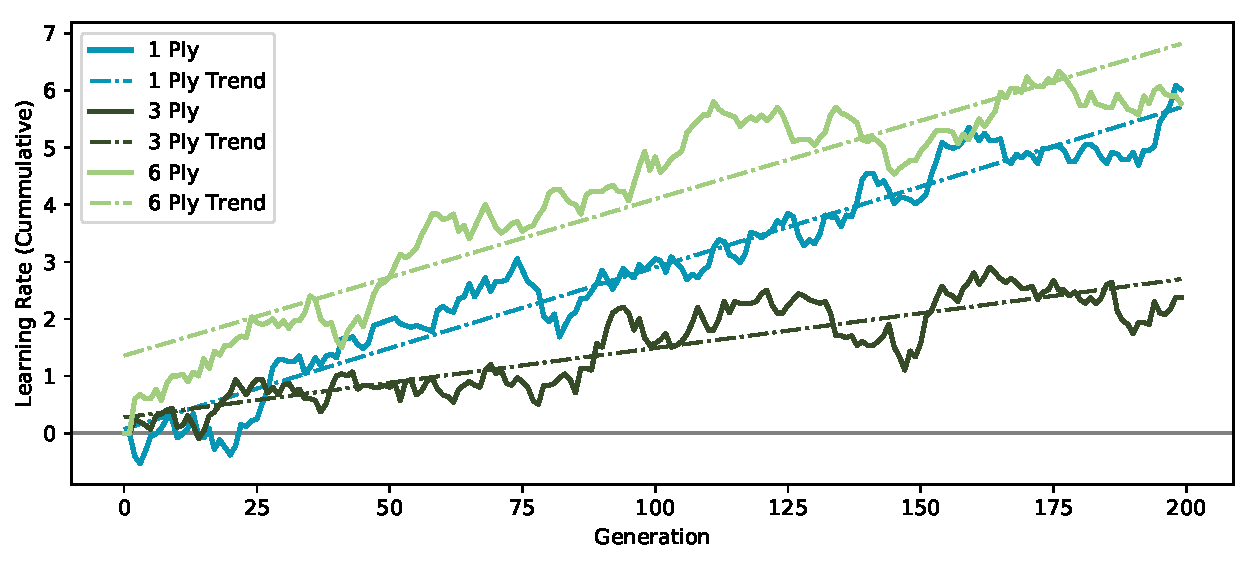
\includegraphics[width=250mm]{images/results/combined_cummulative.pdf}
      \caption{A chart showing the cumulative learning rate across the generations for the different ply-depths.\label{cum_growth}}
    \end{figure}
  \end{frame}
  
  \begin{frame}

    \frametitle{Trained System Statistics} 
    \begin{figure}[!ht]
      \centering
      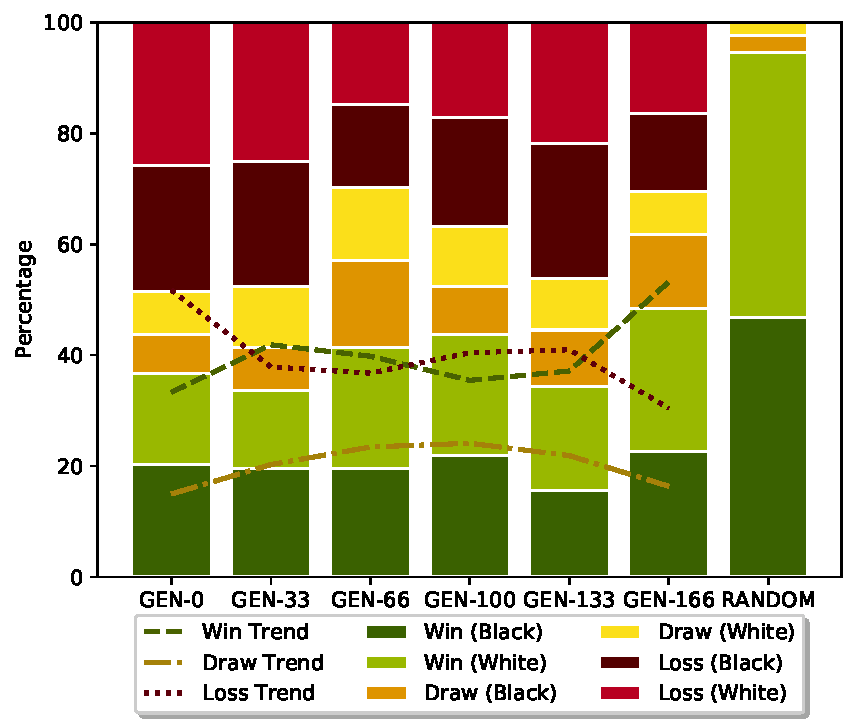
\includegraphics[width=80mm]{images/results/1ply/gm_net_stats.pdf}
      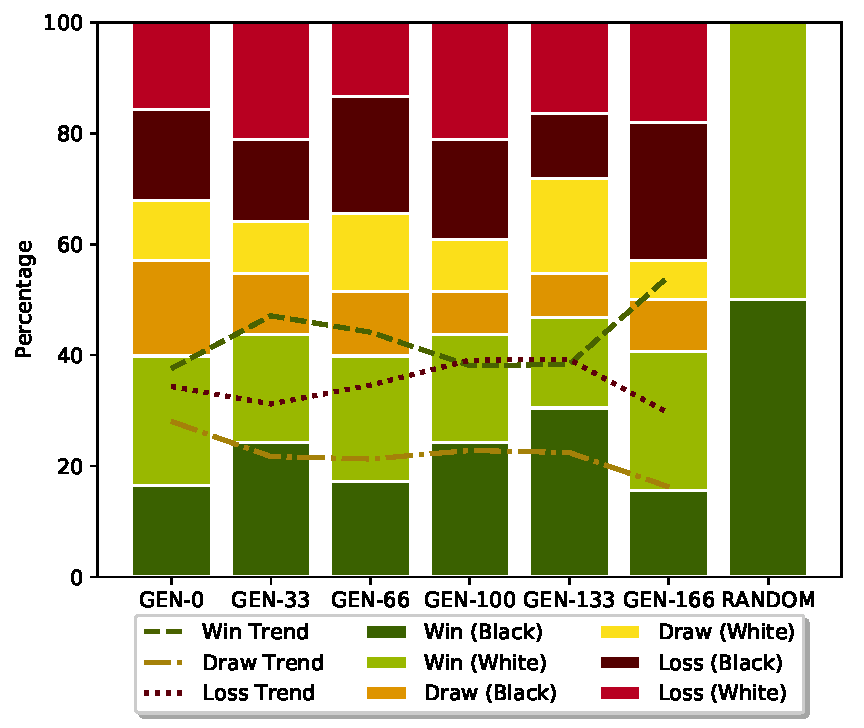
\includegraphics[width=80mm]{images/results/3ply/gm_net_stats.pdf}
      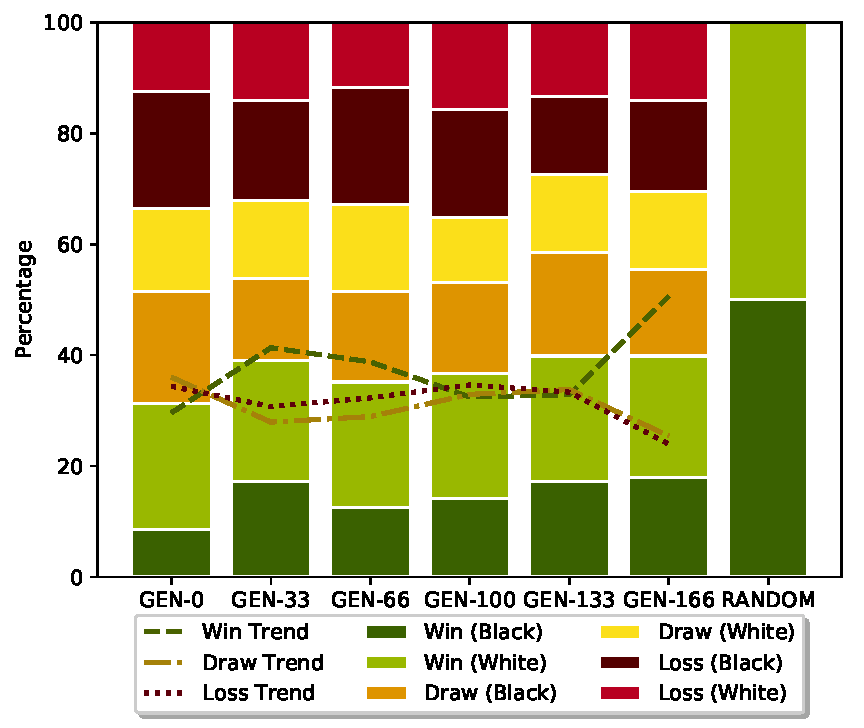
\includegraphics[width=80mm]{images/results/6ply/gm_net_stats.pdf}
      \caption{Charts showing the performance of the trained systems against their ancestral counterparts.\label{net_stats}}
  \end{figure}
  
  \end{frame}

  \begin{frame}

    \frametitle{Champion Genome Distribution} 
    \begin{figure}[!ht]
      \centering
      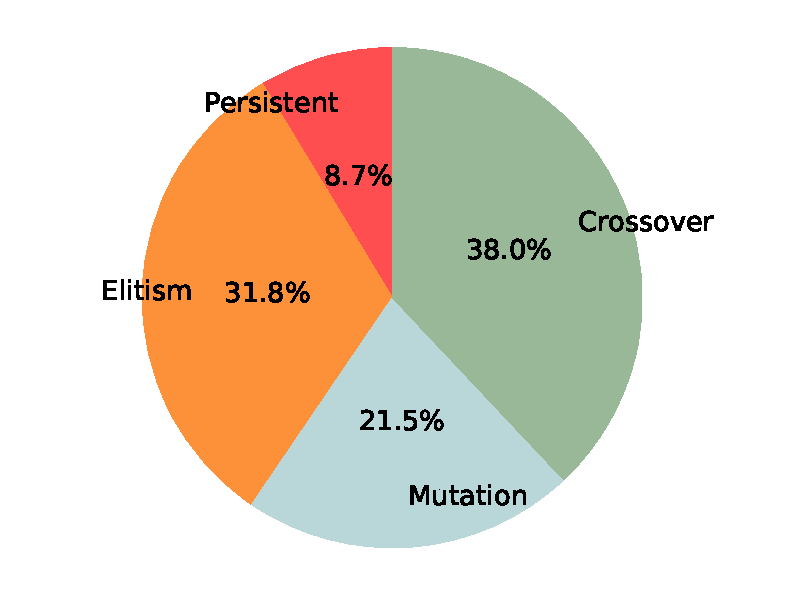
\includegraphics[width=80mm]{images/results/1ply/champ_gen_dist.pdf}
      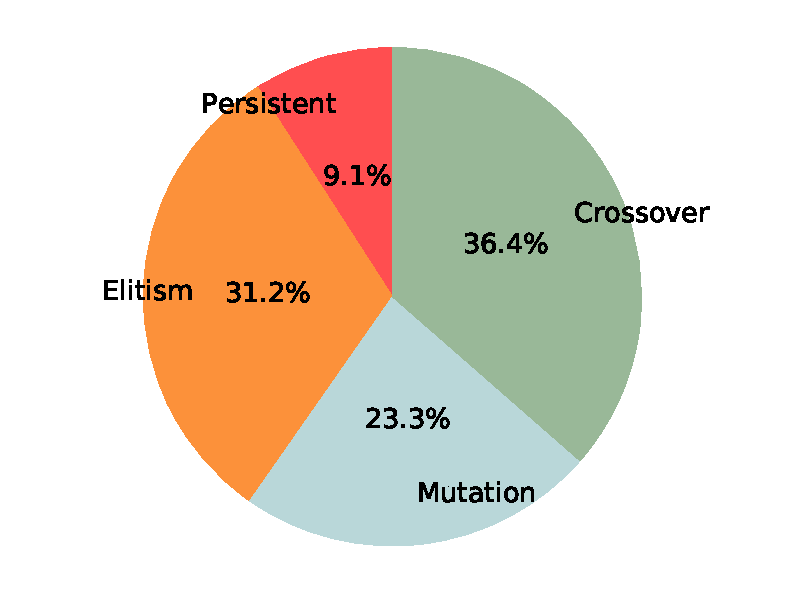
\includegraphics[width=80mm]{images/results/3ply/champ_gen_dist.pdf}
      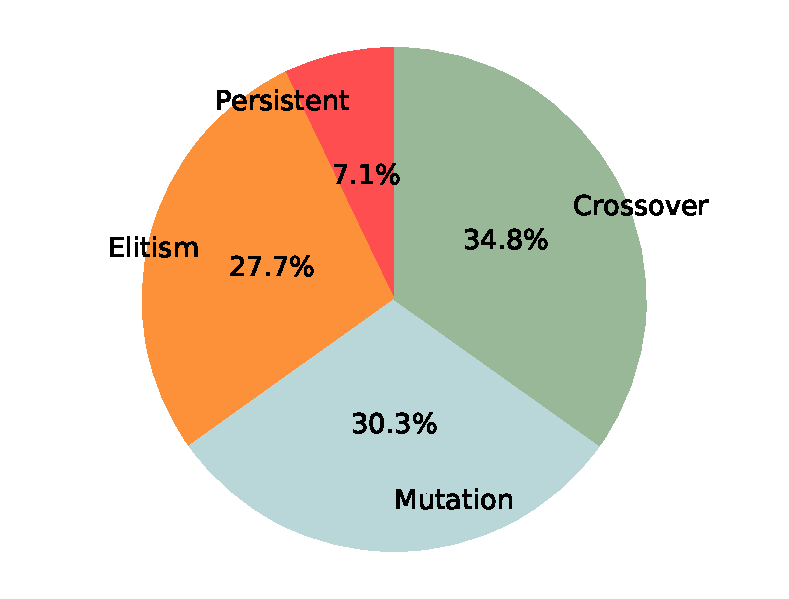
\includegraphics[width=80mm]{images/results/6ply/champ_gen_dist.pdf}
      \caption{Distributions of the different genomic identities across the tournament champions. \label{champ_gen_dist}}
  \end{figure}

  \end{frame}

  \begin{frame}
    \centering
    \frametitle{Score Distribution of Different Champion Genomes} 
    \begin{figure}[!ht]
      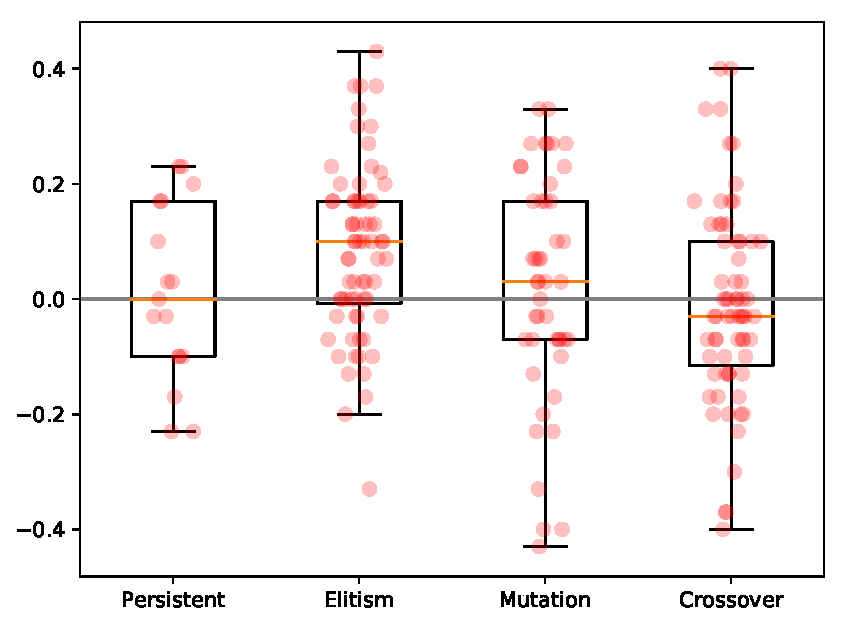
\includegraphics[width=80mm]{images/results/1ply/champ_score_distribution.pdf}
      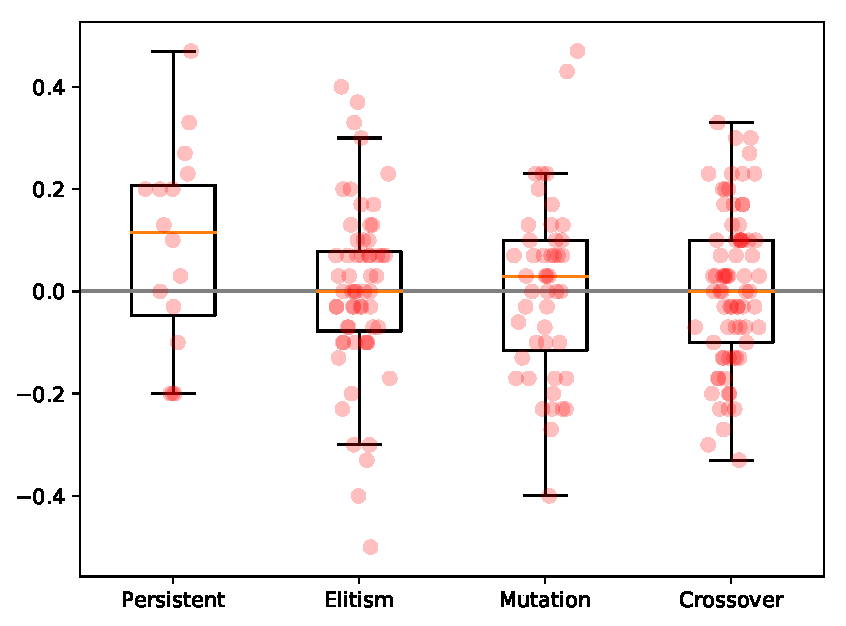
\includegraphics[width=80mm]{images/results/3ply/champ_score_distribution.pdf}
      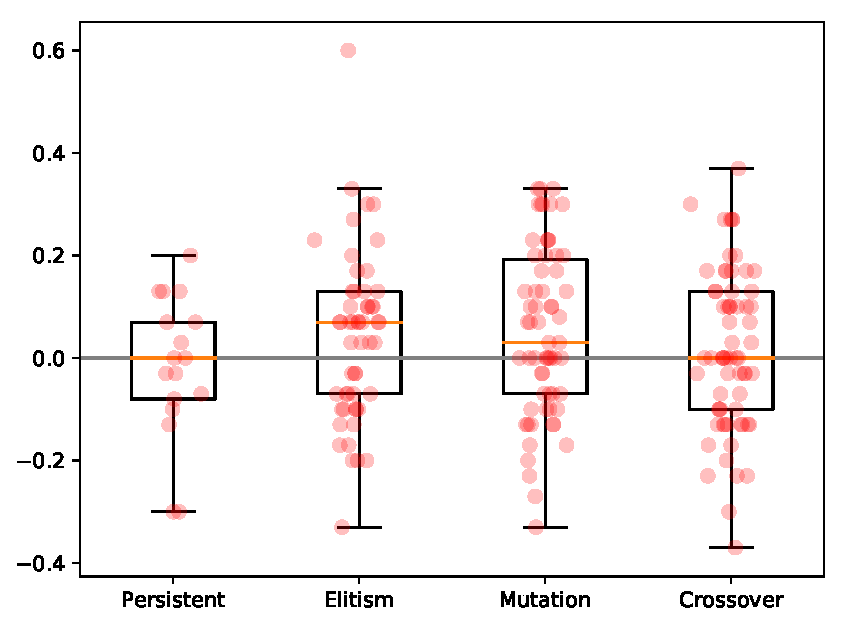
\includegraphics[width=80mm]{images/results/6ply/champ_score_distribution.pdf}
      \caption{Box-Plots of the different genomic identities and their distribution of scores. The yellow line in the box represents the mean score. \label{champ_score_distribution}}
  \end{figure}

  \end{frame}

  \begin{frame}
    \frametitle{Average Move Count} 
    \begin{figure}[!ht]
      \centering
      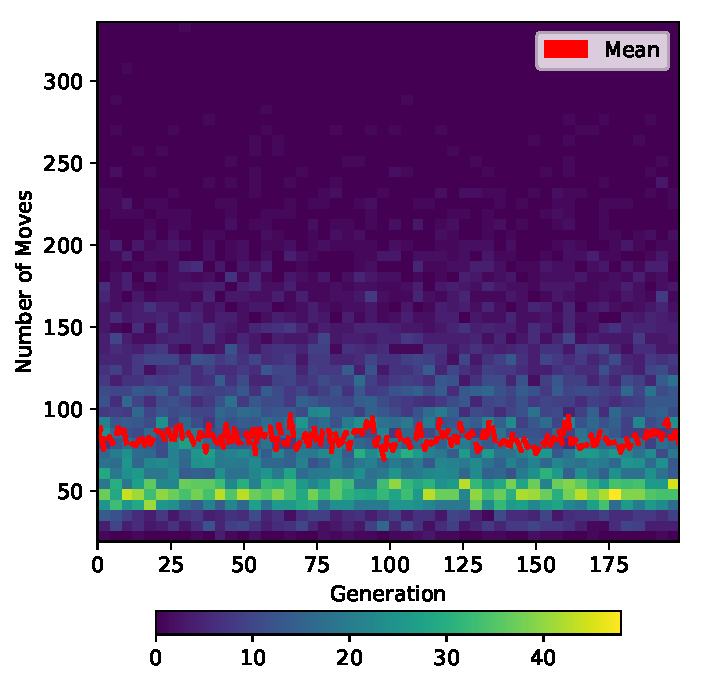
\includegraphics[width=80mm]{images/results/1ply/moves.pdf}
      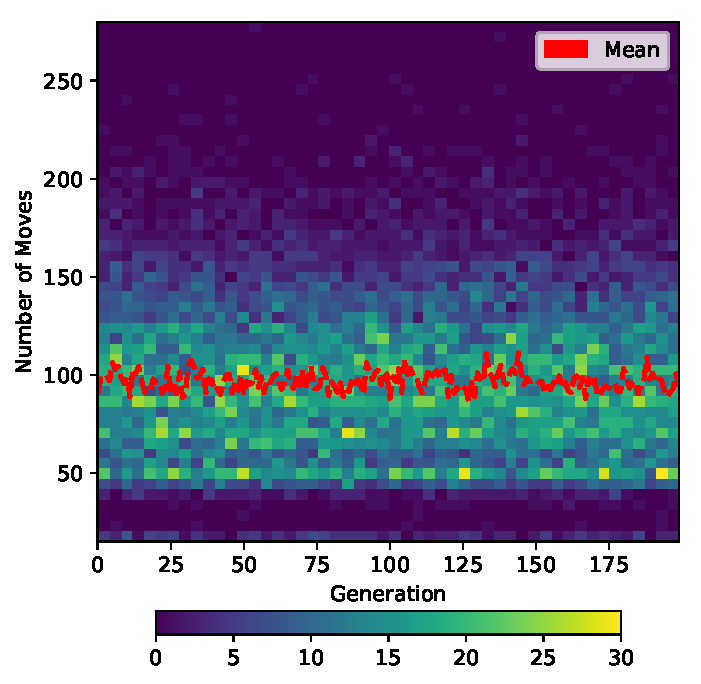
\includegraphics[width=80mm]{images/results/3ply/moves.pdf}
      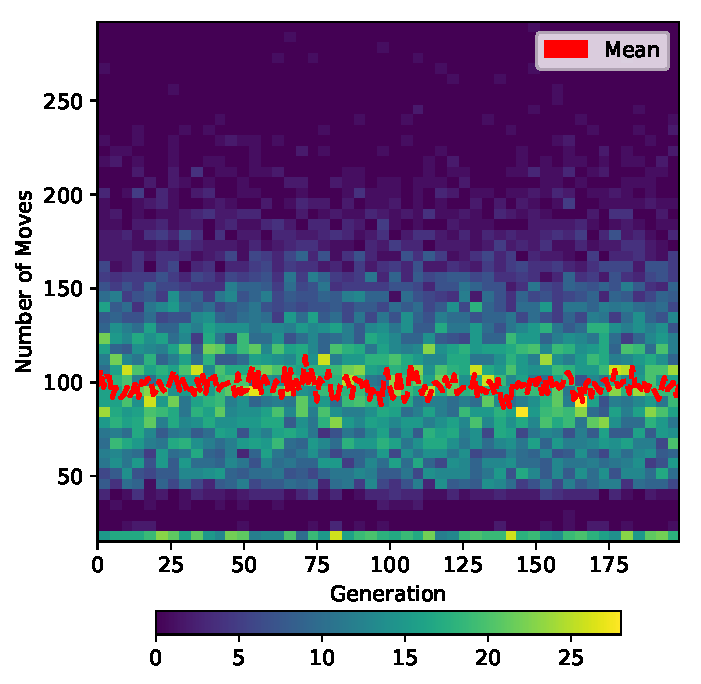
\includegraphics[width=80mm]{images/results/6ply/moves.pdf}
      \caption{2D Histograms representing the number of moves played in the games played in the generations. \label{move_chart}}
  \end{figure}

  \end{frame}

  \begin{frame}
    \frametitle{CPU Timings} 
    \begin{figure}
        \begin{tabular}{ccccc}
          & 1-Ply        & 3-Ply          & 6-Ply          & \\ \cline{2-4}
    \multicolumn{1}{c|}{Generation Mean} & \multicolumn{1}{r|}{0:04:24} & \multicolumn{1}{r|}{0:17:32}  & \multicolumn{1}{r|}{0:38:45}   & \\ \cline{2-4}
    \multicolumn{1}{c|}{Net (All Generations)} & \multicolumn{1}{r|}{7:21:25} & \multicolumn{1}{r|}{1 day, 5:14:41} & \multicolumn{1}{r|}{5 days, 9:12:25} & \\ \cline{2-4}
          &          &           &            & 
    \end{tabular}

    \caption{Mean and Net running times of system training for the various depths. \label{cpu_table}}
    \end{figure}


    \begin{figure}[!ht]
    \centering
    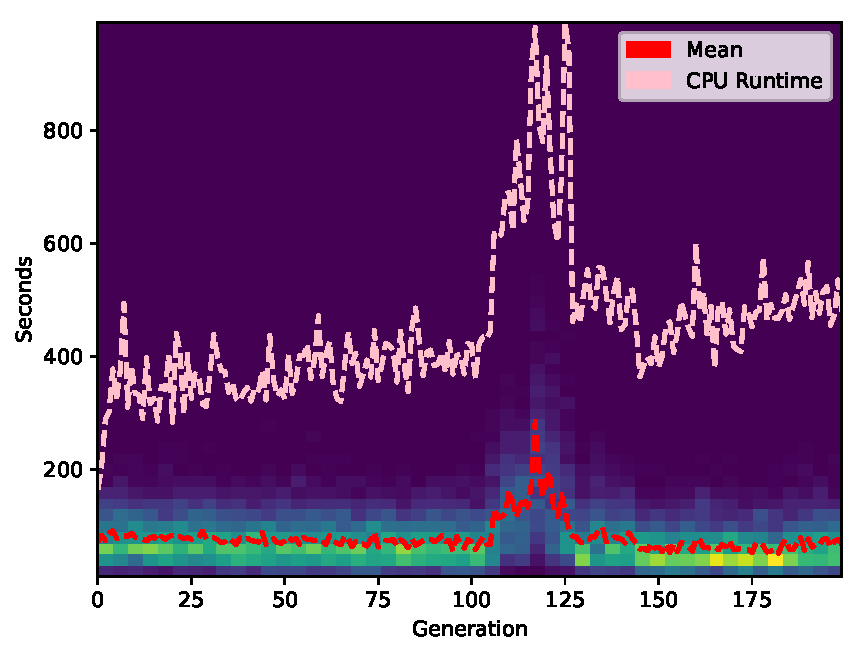
\includegraphics[width=80mm]{images/results/1ply/simulation_timings.pdf}
    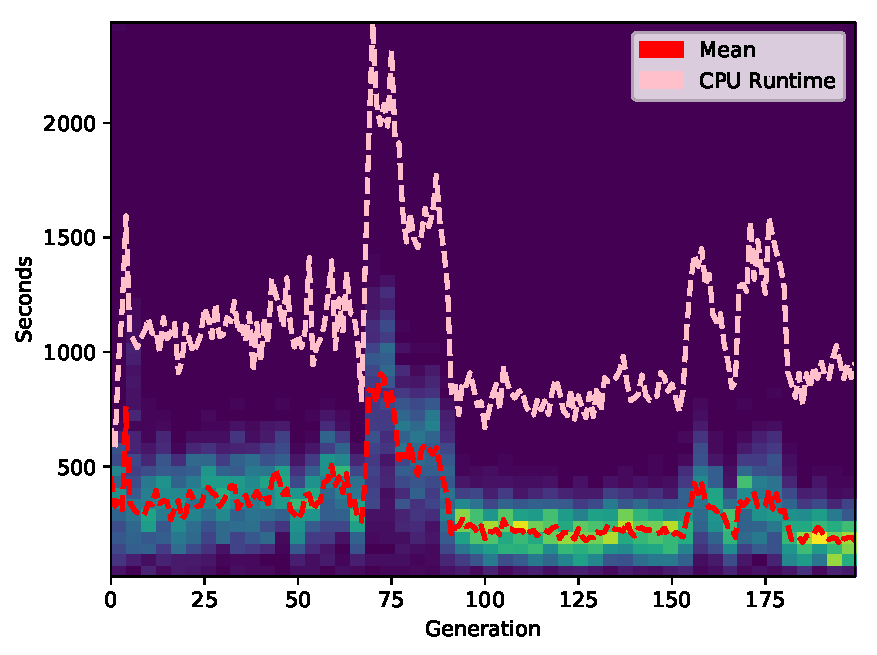
\includegraphics[width=80mm]{images/results/3ply/simulation_timings.pdf}
    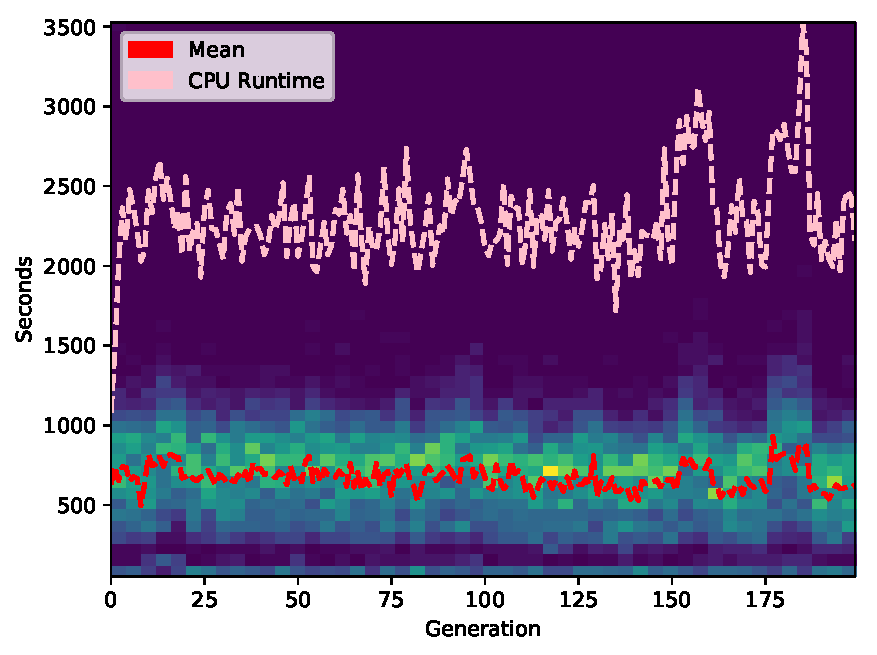
\includegraphics[width=80mm]{images/results/6ply/simulation_timings.pdf}
    \caption{2D Histograms of the average times spent on the games during the simulations. \label{chart_cpu_times}}
    \end{figure}
  \end{frame}
    


\end{document}
  